\documentclass[titlepage, 11pt]{article}
\usepackage[a4paper, total={6in, 9.5in}]{geometry}
\usepackage{graphicx}
\usepackage{amsmath,amsfonts,amssymb}
\usepackage{listings}
\usepackage{booktabs}
\usepackage[T1]{fontenc}
\usepackage{listings}
\usepackage{color}
\usepackage{minted}
\usepackage[colorlinks=true, linkcolor=blue, urlcolor=blue, citecolor=blue, pdfborder={0 0 255}]{hyperref}
\usepackage{colortbl}
\usepackage{url}
\usepackage{xcolor}
\usepackage{caption}
\usepackage{subcaption}
\usepackage{dirtytalk}
\usepackage[semicolon, round]{natbib}
\usepackage[ruled]{algorithm2e}
\usepackage{tabto}
\usepackage{gnuplottex}
\usepackage{avremu}
\usepackage{graphicx}
\graphicspath{ {./images/} }
\captionsetup[table]{skip=10pt}
\renewcommand{\vec}[1]{\mathbf{#1}}
\SetKwComment{Comment}{$\triangleright$\ }{}

\usepackage{tikz}
\usetikzlibrary{shapes.geometric, arrows}
\tikzstyle{startstop} = [rectangle, rounded corners, minimum width=3cm, text width = 3cm, minimum height=1cm,text centered, draw=black, fill=red!30]
\tikzstyle{io} = [trapezium, trapezium left angle=70, trapezium right angle=110, minimum width=2cm, minimum height=1cm, text centered, draw=black, fill=blue!30, text width = 2cm]
\tikzstyle{process} = [rectangle, minimum width=3cm, minimum height=1cm, text width = 5cm, text centered, draw=black, fill=orange!30]
\tikzstyle{decision} = [diamond, minimum width=3cm, minimum height=1cm, text width = 3cm, text centered, draw=black, fill=green!30]
\tikzstyle{arrow} = [thick,->,>=stealth]



% \hypersetup{%
% 	colorlinks=true,
% 	linkcolor=blue,
% 	linkbordercolor={0 0 1}
% }

% \renewcommand\lstlistingname{Algorithm}
% \renewcommand\lstlistlistingname{Algorithms}
% \def\lstlistingautorefname{Alg.}



\newcommand{\argmin}{\mathop{\mathrm{argmin}}}
\newcommand{\argmax}{\mathop{\mathrm{argmax}}}
\newcommand{\minimize}{\mathop{\mathrm{minimize}}}
\newcommand{\maximize}{\mathop{\mathrm{maximize}}}
\newcommand{\st}{\mathop{\mathrm{subject\,\,to}}}
\newcommand{\dist}{\mathop{\mathrm{dist}}}
\newcommand{\norm}[1]{\left\lVert#1\right\rVert}
\renewcommand{\vec}[1]{\mathbf{#1}}

\newenvironment{qanda}{\setlength{\parindent}{0pt}}{\bigskip}
\newcommand{\Q}{\bigskip\textbf{Q:} }
\newcommand{\A}{\par\textbf{A:} \normalfont}

\def\R{\mathbb{R}}
\def\E{\mathbb{E}}
\def\P{\mathbb{P}}
\def\S{\mathbb{S}}
\def\Cov{\mathrm{Cov}}
\def\Var{\mathrm{Var}}
\def\half{\frac{1}{2}}
\def\quat{\frac{1}{4}}
\def\sign{\mathrm{sign}}
\def\supp{\mathrm{supp}}
\def\th{\mathrm{th}}
\def\tr{\mathrm{tr}}
\def\dim{\mathrm{dim}}
\def\dom{\mathrm{dom}}


\title{
{EE2016: Microprocessor Lab} \\~\\
{\vlarge Experiment 9: Interrupts in Atmel AVR Atmega through Assembly Programming}\\
}\author{Ajeet E S, EE22B086
    & Amogh Agrawal, EE22B087
}
%\date{27 September, 2023}

\begin{document}
\maketitle
\setcounter{page}{0}
\tableofcontents
\listoflistings
\newpage


\section{Aim}
Using Atmel AVR assembly language programming, implement interrupts and DIP switches control in Atmel Atmega microprocessor. 
\\
\\Aims of this experiment are:

\begin{enumerate}

\item Generate an external (logical) hardware interrupt using an emulation of a push button switch.

\item Write an ISR (Interrupt Service Routine) to switch ON an LED for a few seconds (10 secs) and then switch OFF. (The lighting of the LED could be verifed by monitoring the signal to switch it ON).

\item If there is time, you could try this also: Use the 16 bit timer (via interrupt) to make an LED blink with a duration of 1 second.

\end{enumerate}

Also, one needs to implement all of the above, in AVR assembly.

\section{Observations and Code: Google Drive Link}
The link to the codes and video for the Experiment are uploaded here:

\href{https://drive.google.com/drive/folders/1Gw2JlWqYw3BulAckZvRAgrL_ntPiwJyt?usp=sharing} {Code and Video}


\section{Problem 1: Implement Interrupt using INT1} 

\subsection{Problem Statement}
You are given the file "EE2016F23Exp9int1.asm" which is an assembly program which implements interrupt using INT1. Fill in the blanks in the assembly code.

\subsection{Approach}
\begin{itemize}
\item The ISR for INT1 is set at the label int1\_ISR by using the following command (ISR for INT1 is set in the memory address 0x04):
{\renewcommand\fcolorbox[4][]{\textcolor{black}{\strut#4}}
\begin{minted}{asm}
    .ORG 0x0004 ;
    RJMP int1_ISR;
\end{minted}
}

\item At the program origin, we make the program jump to the label reset. Here, the following are done:

    \begin{enumerate}
        \item Store the memory address of RAMEND to Stack Pointer.
        \item Make PB1 as output and make all of PortD as input and take the input from PIND3, enabling internal pull-up resistor.
        \item Set ISC11 in MCUCR to 1, that is, make a falling edge of interrupt pin generate an interrupt.
        \item Enable Interrupt for INT1 in GICR.
        \item Enable all interrupts using SEI.
    \end{enumerate}

\item The program waits at the label "indefiniteloop", waiting for an interrupt:
    {\renewcommand\fcolorbox[4][]{\textcolor{black}{\strut#4}}
    \begin{minted}{asm}
    indefiniteloop: RJMP indefiniteloop
    \end{minted}
}

\item In the "int1\_ISR" Routine, the LED is made to blink 10 times with the duty cycle as given in the code.
\end{itemize}


\subsection{Flowchart}
\begin{center}
    

\begin{tikzpicture}[node distance=2cm]
\node (start) [startstop , xshift = -2cm] {Start};
\node (pro1) [process, right of=start, xshift=3cm] {Set the .org 0x00 Rjmp Reset\\ and .org 0x0004};
\node (pro2) [process, right of=pro1, xshift= 4cm] {Reach .org 0x0004 for Rjmp int1 subroutine};
\node (pro7) [process, below of=pro2, xshift=-6cm, yshift = -.5cm] {Jump to Reset and \\Set up Stack Pointer};

\node (pro3) [process, left of=pro7, xshift=-4cm] {Make PB1 as output and PORTD as input};
\node (pro8) [process, below of=pro3, yshift=-.5cm] {Enable the Pull Up resistor for the PIND3};
\node (pro4) [process, right of=pro8, xshift=4cm] {Setting up ISC11 in MCUCR as 1 and Enabling INT1 in GICR};
\node (pro5) [process, below of=pro4, yshift=-.5cm] {Enable GLobal Interrupt and wait for Interrupt};
\node (in1) [io, below of=pro5, yshift = -.5cm] {Input at PIND3};

\node (pro6) [process, below of=pro2, yshift=-.5cm] {Coding the ISR to ouptut a LED Blinking with Time Period $=$ 0.39sec};
\node (pro9) [process, below of=pro6, yshift=-.5cm] {Excecute the ISR};


\draw [arrow] (start) -- (pro1);
\draw [arrow] (pro1) -- (pro7);
\draw [arrow] (pro7) -- (pro3);
\draw [arrow] (pro3) -- (pro8);
\draw [arrow] (pro8) -- (pro4);
\draw [arrow] (pro4) -- (pro5);
\draw [arrow] (pro5) -- (in1);
\draw [arrow] (pro6) -- (pro9);


\draw [arrow] (pro2) -- (pro6);
\draw [arrow] (in1.south) -- ++(0,-1.5) -- node[anchor=south]{If Input at PIND3$=$1}++(-4,0) |- (pro5.west);
\draw [arrow] (in1.east) -- node[anchor=south]{If Input at PIND3$=$0}++(8,0) |- (pro2.east);
\draw [arrow] (pro9.south) |- (pro5.east);

\end{tikzpicture}
\end{center}

\subsection{Code}
The code is given below:

{\renewcommand\fcolorbox[4][]{\textcolor{black}{\strut#4}}
\inputminted[breaklines,
 mathescape,
 linenos,
 numbersep=5pt,
 frame=single,
 numbersep=5pt,
 xleftmargin=0pt]{asm}{"Prob1.asm"}}
\captionof{listing}{Code to Blink LED using INT1}

\subsection{Questions From Code}
\begin{qanda}

\Q \mintinline{asm}{LDI R16, HIGH(RAMEND);} Guess, why it is done ???
\A This is store the top 8 bits of the address of the end of data memory.

\Q {\renewcommand\fcolorbox[4][]{\textcolor{black}{\strut#4}}\mintinline{asm}{ORI R16, 1<< ISC11;}} Why it is Ored?
\A It is Ored to not change the rest of the bits of R16 except the bit at the same position as that of ICS11 in the MCUCR which is set to 1. 

\Q\mintinline{asm}{ SEI;} What does it do?
\A It sets the global interrupt enable in SREG Register as 1.

\Q \mintinline{asm}{indefiniteloop: rjmp indefiniteloop;} Stay here. Expecting interrupt? 
\A Yes. The program stays here, waiting for an interrupt.

\Q What is the Duty Cycle and period of the LED Blinking?
\A Duty cycle is 50\%  while the LED blinking period is 390158 cycles, equivalent to  .39sec.

\end{qanda}


\subsection{Inferences}

\subsubsection{Interrupts}
\begin{itemize}
    \item It is a method used to serve a device using a microcontroller.
    \item In this, the device sends an interrupt signal to the microcontroller, upon which the microcontroller pauses all other processes and serves the device.
    \item This is better than Polling, in which the microcontroller keeps monitoring the output of a device in the fact that it doesn't waste time monitoring all devices, and makes the rest of the program wait only when a request is made.
\end{itemize}

\subsubsection{Interrupt Service Routine(ISR):}
\begin{itemize}
    \item The ISR is the Routine that is called when an interrupt is raised. 
    \item This routine is called only if Global Interrupt Enable is set using the SEI Command
    \item When an interrupt request occurs for INT1, the program goes to the memory address 0x04, the interrupt vector for the same
\end{itemize}

\subsubsection{Interrupt Vector:}
\begin{itemize}
    \item The Microcontroller checks in a memory address called Interrupt Vector, to find the memory address at which the ISR is stored.
    \item The Interrupt Vectors for INT0, INT1 and INT2 are memory addresses 0x02,0x04 and 0x06
    \item Whenever an Interrupt occurs, the program goes to these memory addresses and searches for the memory address for the ISR.
\end{itemize}

\subsubsection{Taking Care of Interrupts}
Whenever an Interrupt Signal is received, the microcontroller does the following:
    \begin{enumerate}
        \item Finishes the instruction it is currently executing and store the address of the next instruction in the PC.
        \item Jumps to the Interrupt Vector Table, which redirects the microcontroller to the ISR.
        \item Executes the ISR until it encounters RETI, upon which it goes to the next instruction to be executed and continues normally.
    \end{enumerate}

\subsubsection{Enabling Interrupts and Choosing Interrupt Signal}
The following are important Registers in relation to Interrupts:

\begin{enumerate}
    \item \textbf{SREG: Status Register}
    \begin{figure}[H]
        \centering
        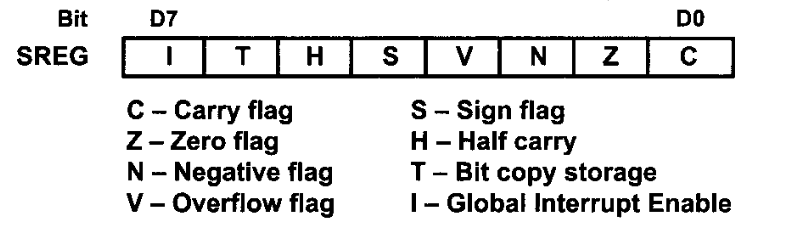
\includegraphics[width=0.75\linewidth]{SREG.png}
    \end{figure}
        \begin{itemize}
            \item Global Interrupt Enable (I), the $7^{th}$ bit, must be set for all interrupts to be accepted.
        \end{itemize}
    
    
    \item \textbf{MCUCR: MCU Control Register}
    \begin{figure}[H]
        \centering
        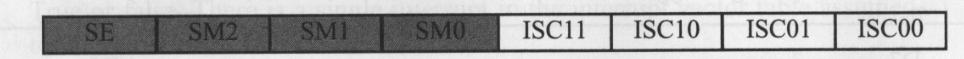
\includegraphics[width=1\linewidth]{MCUCR.png}  
    \end{figure}
        \begin{itemize}
            \item The values of ISC11, ISC10, ISC01, ISC00 and the purposes are given below:
            \begin{figure}[H]
                \centering
                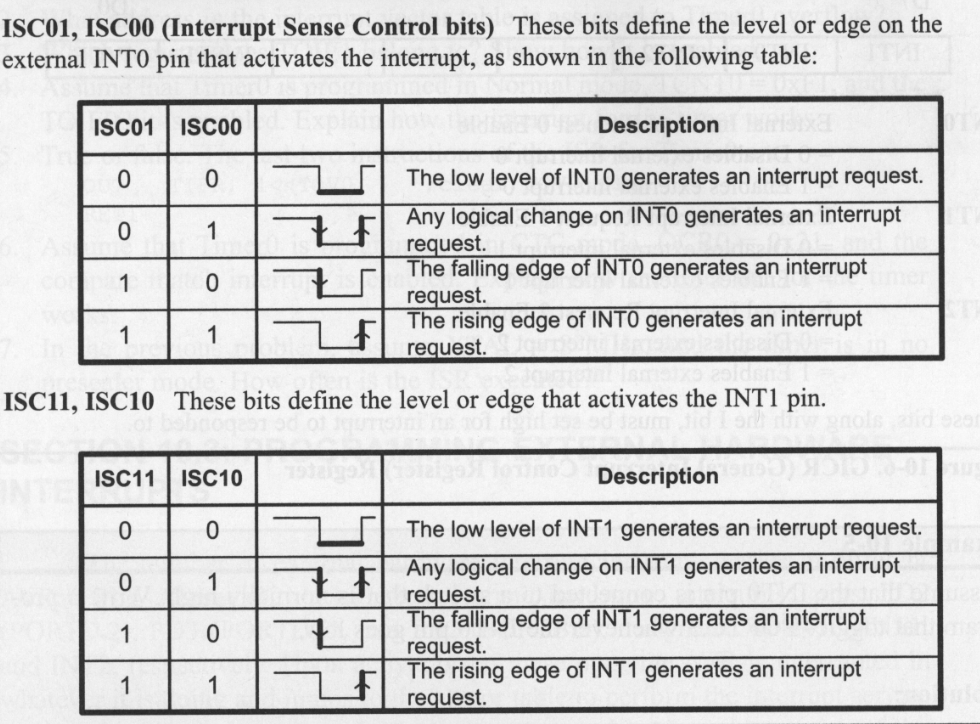
\includegraphics[width=0.8\linewidth]{INT0_and_INT1.png}
            \end{figure}
        \end{itemize}
    
    \item \textbf{MCUCSR: MCU Control and Status Register}
        \begin{itemize}
            \item The value of ISC2 in this register. This bit is used to choose which level and edge is taken as an interrupt.
            \begin{figure}[H]
                \centering
                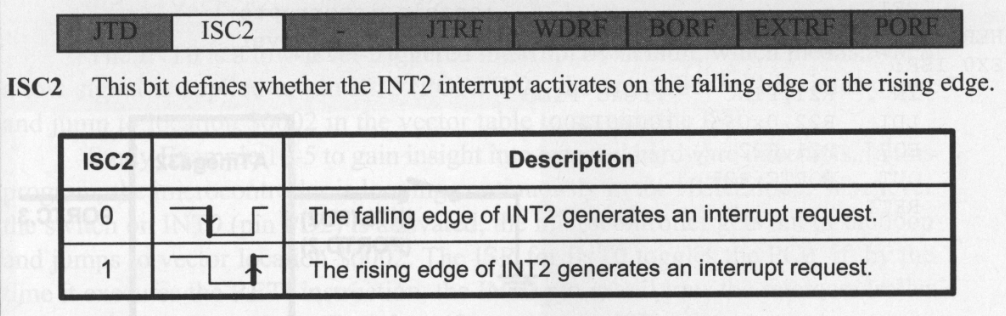
\includegraphics[width=1\linewidth]{MCUCSR.png}
            \end{figure}
        \end{itemize}        
\end{enumerate}

\section{Problem 2: Implement Interrupt using INT0} 

\subsection{Problem Statement}
Perform 4-bit addition of two unsigned nibbles from an 8-bit dip input switch (set by TAs) and display the result obtained in LEDs.

\subsection{Approach}
Essentially, this code uses the same logic as the previous one, but the only difference is that this operates on INT0 and not INT1.

\begin{itemize}
\item The ISR for INT0 is set at the label int0\_ISR by using the following command (ISR for INT0 is set in the memory address 0x02):
{\renewcommand\fcolorbox[4][]{\textcolor{black}{\strut#4}}
\begin{minted}{asm}
    .ORG 0x0002 ;
    RJMP int0_ISR;
\end{minted}
}

\item At the program origin, we make the program jump to the label reset. Here, the following are done:

    \begin{enumerate}
        \item Store the memory address of RAMEND to Stack Pointer.
        \item Make PB1 as output and make all of PortD as input and take the input from PIND2, enabling internal pull-up resistor.
        \item Set ISC01 in MCUCR to 1, that is, make a falling edge of interrupt pin generate an interrupt.
        \item Enable Interrupt for INT0 in GICR.
        \item Enable all interrupts using SEI.
    \end{enumerate}

\item The program waits at the label "indefiniteloop", waiting for an interrupt:
    {\renewcommand\fcolorbox[4][]{\textcolor{black}{\strut#4}}
    \begin{minted}{asm}
    indefiniteloop: RJMP indefiniteloop
    \end{minted}
}

\item In the "int0\_ISR" Routine, the LED is made to blink 10 times
\end{itemize}

\subsection{Flowchart}
\begin{center}
    

\begin{tikzpicture}[node distance=2cm]
\node (start) [startstop , xshift = -2cm] {Start};
\node (pro1) [process, right of=start, xshift=3cm] {Set the .org 0x00 Rjmp Reset\\ and .org 0x0002};
\node (pro2) [process, right of=pro1, xshift= 4cm] {Reach .org 0x0002 for Rjmp int1 subroutine};
\node (pro7) [process, below of=pro2, xshift=-6cm, yshift = -.5cm] {Jump to Reset and \\Set up Stack Pointer};

\node (pro3) [process, left of=pro7, xshift=-4cm] {Make PB1 as output and PORTD as input};
\node (pro8) [process, below of=pro3, yshift=-.5cm] {Enable the Pull Up resistor for the PIND2};
\node (pro4) [process, right of=pro8, xshift=4cm] {Setting up ISC01 in MCUCR as 1 and Enabling INT0 in GICR};
\node (pro5) [process, below of=pro4, yshift=-.5cm] {Enable GLobal Interrupt and wait for Interrupt};
\node (in1) [io, below of=pro5, yshift = -.5cm] {Input at PIND2};

\node (pro6) [process, below of=pro2, yshift=-.5cm] {Coding the ISR to ouptut a LED Blinking with Time Period $=$ 0.39sec};
\node (pro9) [process, below of=pro6, yshift=-.5cm] {Excecute the ISR};


\draw [arrow] (start) -- (pro1);
\draw [arrow] (pro1) -- (pro7);
\draw [arrow] (pro7) -- (pro3);
\draw [arrow] (pro3) -- (pro8);
\draw [arrow] (pro8) -- (pro4);
\draw [arrow] (pro4) -- (pro5);
\draw [arrow] (pro5) -- (in1);
\draw [arrow] (pro6) -- (pro9);


\draw [arrow] (pro2) -- (pro6);
\draw [arrow] (in1.south) -- ++(0,-1.5) -- node[anchor=south]{If Input at PIND2$=$1}++(-4,0) |- (pro5.west);
\draw [arrow] (in1.east) -- node[anchor=south]{If Input at PIND2$=$0}++(8,0) |- (pro2.east);
\draw [arrow] (pro9.south) |- (pro5.east);

\end{tikzpicture}
\end{center}

\subsection{Code}
The code to perform 4- bit addition is given below:

{\renewcommand\fcolorbox[4][]{\textcolor{black}{\strut#4}}
\inputminted[breaklines,
 mathescape,
 linenos,
 numbersep=5pt,
 frame=single,
 numbersep=5pt,
 xleftmargin=0pt]{asm}{"Prob2.asm"}}
\captionof{listing}{Code to Blink LED using INT0}


\subsection{Questions From Code}
\begin{qanda}

\Q \mintinline{asm}{LDI R16, HIGH(RAMEND);} Guess, why it is done ???
\A This is store the top 8 bits of the address of the end of data memory.

\Q {\renewcommand\fcolorbox[4][]{\textcolor{black}{\strut#4}}\mintinline{asm}{ORI R16, 1<< ISC01;}} Why it is Ored?
\A It is Ored to not change the rest of the bits of R16 except the bit at the same position as that of ICS11 in the MCUCR which is set to 1. 

\Q\mintinline{asm}{ SEI;} What does it do?
\A It sets the global interrupt enable in SREG Register as 1.

\Q \mintinline{asm}{indefiniteloop: rjmp indefiniteloop;} Stay here. Expecting interrupt? 
\A Yes. The program stays here, waiting for an interrupt.

\Q What is the Duty Cycle and period of the LED Blinking?
\A Duty cycle is 50\%  while the LED blinking period is 390158 cycles, equivalent to  .39sec.

\end{qanda}

\subsection{Inferences}

\subsubsection{Interrupts}
\begin{itemize}
    \item It is a method used to serve a device using a microcontroller.
    \item In this, the device sends an interrupt signal to the microcontroller, upon which the microcontroller pauses all other processes and serves the device.
    \item This is better than Polling, in which the microcontroller keeps monitoring the output of a device in the fact that it doesn't waste time monitoring all devices, and makes the rest of the program wait only when a request is made.
\end{itemize}

\subsubsection{Interrupt Service Routine(ISR):}
\begin{itemize}
    \item The ISR is the Routine that is called when an interrupt is raised. 
    \item This routine is called only if Global Interrupt Enable is set using the SEI Command
    \item When an interrupt request occurs for INT1, the program goes to the memory address 0x04, the interrupt vector for the same
\end{itemize}

\subsubsection{Interrupt Vector:}
\begin{itemize}
    \item The Microcontroller checks in a memory address called Interrupt Vector, to find the memory address at which the ISR is stored.
    \item The Interrupt Vectors for INT0, INT1 and INT2 are memory addresses 0x02,0x04 and 0x06
    \item Whenever an Interrupt occurs, the program goes to these memory addresses and searches for the memory address for the ISR.
\end{itemize}

\subsubsection{Taking Care of Interrupts}
Whenever an Interrupt Signal is received, the microcontroller does the following:
    \begin{enumerate}
        \item Finishes the instruction it is currently executing and store the address of the next instruction in the PC.
        \item Jumps to the Interrupt Vector Table, which redirects the microcontroller to the ISR.
        \item Executes the ISR until it encounters RETI, upon which it goes to the next instruction to be executed and continues normally.
    \end{enumerate}

\subsubsection{Enabling Interrupts and Choosing Interrupt Signal}
The following are important Registers in relation to Interrupts:

\begin{enumerate}
    \item \textbf{SREG: Status Register}
    \begin{figure}[H]
        \centering
        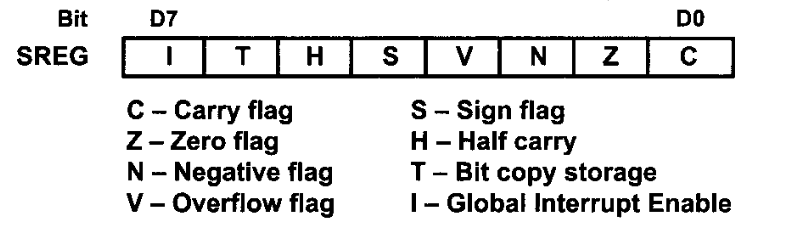
\includegraphics[width=0.75\linewidth]{SREG.png}
    \end{figure}
        \begin{itemize}
            \item Global Interrupt Enable (I), the $7^{th}$ bit, must be set for all interrupts to be accepted.
        \end{itemize}
    
    
    \item \textbf{MCUCR: MCU Control Register}
    \begin{figure}[H]
        \centering
        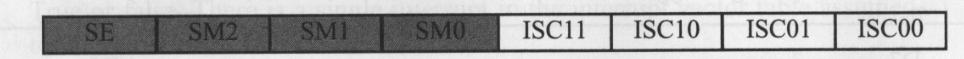
\includegraphics[width=1\linewidth]{MCUCR.png}  
    \end{figure}

        \begin{itemize}
            \item The values of ISC11, ISC10, ISC01, ISC00 and the purposes are given below:
            \begin{figure}[H]
                \centering
                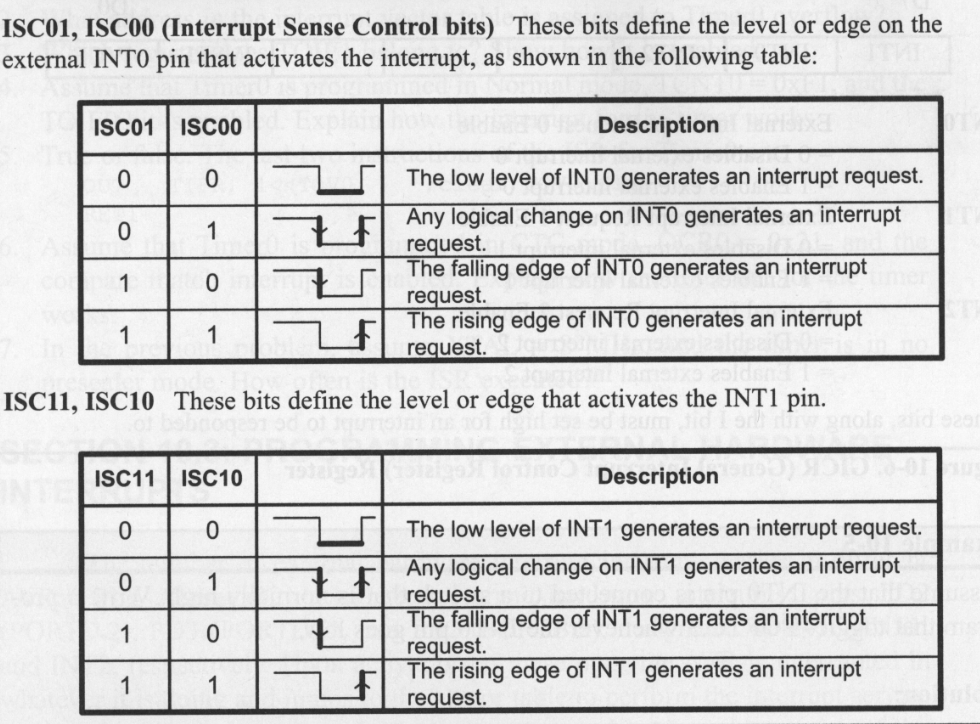
\includegraphics[width=0.8\linewidth]{INT0_and_INT1.png}
            \end{figure}
        \end{itemize}
    
    \item \textbf{MCUCSR: MCU Control and Status Register}
        \begin{itemize}
            \item The value of ISC2 in this register. This bit is used to choose which level and edge is taken as an interrupt.
            \begin{figure}[H]
                \centering
                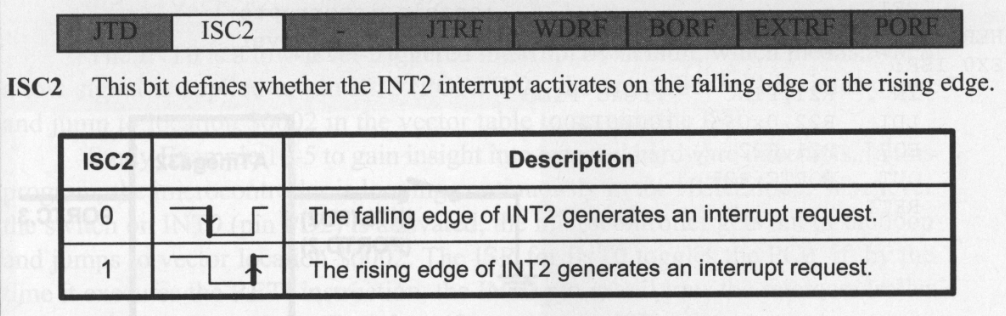
\includegraphics[width=1\linewidth]{MCUCSR.png}
            \end{figure}
        \end{itemize}
\end{enumerate}

\end{document}